\documentclass[a4paper,twocolumn]{article}
\pagestyle{empty}

\usepackage[portuguese]{babel}
\usepackage[T1]{fontenc}
\usepackage[utf8]{inputenc}
\usepackage{amsfonts}
%\usepackage{concmath}

\usepackage{booktabs}
\renewcommand{\arraystretch}{1.2}

%\usepackage{natbib}
%\usepackage{pstricks}
%\usepackage{pst-plot}
\usepackage[pdftex]{graphicx}
\usepackage{url}
%\usepackage[top=1cm,bottom=1cm,left=1cm,right=1cm]{geometry}
%\usepackage{multicol}

%\usepackage{amssymb,amsmath}
%\usepackage{extraipa}
%\usepackage{euler}
%\everymath{\displaystyle}

\author{André Wagner}
\title{Análise do Problema da Mochila}
\date{}

\begin{document}

\maketitle

%%%%%%%%%%%%%%%%%%%%%%%%%%%%%%%%%%%%%%%%%%%%%%%%%%%%%%%%%%%%%%%%

\section{Introdução}

Teoria da complexidade computacional\cite{sipser05} é um ramo da ciência da computação que se ocupa com o estudo e a classificação de algoritmos computacionais de acordo com a sua complexidade. Os problemas são separados em \emph{classes de complexidade}, que compõe conjuntos de algoritmos de complexidade relacionadas. 

A análise de um algoritmo é realizada através da sua taxa de crescimento relacionada ao tamanho de sua entrada. O crescimento avaliado pode ser por processamento ou uso de memória, embora o processamento geralmente seja a medida utiliada. Uma algoritmo, por exemplo, que dobra o tempo de processamento a cada aumento simples de sua entrada é chamado quadrático, pois para uma entrada de tamanho $n$ o tempo de processamento leva $n^2$. Na avaliação, geralmente é utilizado o pior caso.

A notação utilizada para a representação da complexidade de um algoritmo é a \emph{notação assintótica} (também conhecida como Grande-O). Esta notação caracteriza uma função de acordo com o seu crescimento. Numa descrição informal, pode-se afirmar que a notação leva sempre em consideração o maior termo de uma função. Por exemplo: se o crescimento do tempo de execução de um algoritmo em relação ao tempo for representado pela função $f(n) = \frac{1}{2}n^3 + 14n^2 - 150n$, diz-se que este algoritmo tem complexidade $O(n^3)$, uma vez que $n^3$ é o maior termo da função.

Dentre as diversas classes de complexidade, algumas das mais importantes e mais utilizadas são as classes DTIME, P, EXPTIME, NP, PSPACE e L. Para o objeto de estudo deste trabalho, serão analisadas as classes P e NP.

% TODO - descrever seções

%%%%%%%%%%%%%%%%%%%%%%%%%%%%%%%%%%%%%%%%%%%%%%%%%%%%%%%%%%%%%%%%

\section{Classes P e NP}

A classificação das classes computacionais é feita levando-se em consideração o recurso de tempo ou memória necessários para se resolver um problema de decisão em uma determinada máquina. Um problema de decisão é um problema que pode ser resolvido com uma resposta ``sim'' ou ``não''. Por exemplo: ``dado um número $x$, a raiz quadrada de $a$ resulta em um inteiro?''

Para efeito desta discussão, uma máquina abstrata pode ser uma máquina de Turing determinístia ou não-determinística. Uma máquina de Turing determinística é aquela onde existe um conjunto de regras descreve uma única ação que pode ser tomada para uma determinada situação. Já uma máquina de Turing não-determinística possui mais de uma ação que pode ser tomada para cada situação, todas estas ações simultaneamente. Um exemplo de um algoritmo executado em uma máquina de Turing não-deterministica poderia ser um algoritmo de ordenação, onde cada ação seria ordenar a lista de uma forma diferente. Como uma das ordenações seria eventualmente a correta, e todas as ordenações são feitas ao mesmo tempo, este algoritmo executaria em tempo $O(1)$.

Enquanto o máquina de Turing determinística possui sua contrapartida física (exceto pela fita infinita), a máquina de Turing não-determinística é uma máquina teórica utilizada para a classificação de algoritmos.

O conjunto de problemas da \textbf{classe P} contém todos os problemas de decisão que podem ser resolvidos por uma máquina de Turing determinística utilizando tempo polinomial. Um algoritmo pode ser resolvido em tempo polinomial caso ele possa ser resolvido em $O(n^k)$, onde $k$ é uma constante. Problemas de tempo polinomial podem ser resolvidos de forma rápida ou eficiente.

O conjunto de problemas da \textbf{classe NP} contém os todos os problemas de decisão que podem ser resolvidos por uma máquina de Turing não-determinística utilizando tempo polinomial. A solução dos problemas da classe NP podem ser \emph{verificados em tempo polinomial} por uma máquina de Turing deteminística. 

A classe P está contida na classe NP, mas é desconhecido se todos os problemas da classe NP estão contidos em P (ou seja, se $P=NP$), que é a questão aberta mais importante na ciência da computação hoje. Os problemas para os quais não se achou uma solução polinomial determinística são chamados de problemas NP-completos. Isto é ilustrado na Figura~\ref{fig:complexity}.

\begin{figure}
  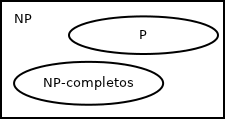
\includegraphics[width=0.5\textwidth]{complexity.png}
  \caption{Diagrama das classes de complexidade se $P\neq NP$.}
  \label{fig:complexity}
\end{figure}

Alguns problemas clássicos da classe NP-Completo são: o problema de satisfabilidade booleana, o jogo dos 15, o problema da mochila, o caminho hamiltoneano, o problema do caixeiro viajante, o problema da coloração de mapas, entre outros. A próxima seção discute o problema da mochila.

%%%%%%%%%%%%%%%%%%%%%%%%%%%%%%%%%%%%%%%%%%%%%%%%%%%%%%%%%%%%%%%%

\section{O problema da mochila}

A origem do problema da mochila é desconhecido. Os trabalhos mais antigos tratando deste problema datam de 1897.

O problema da mochila pode ser descrito informalmente a partir do seguinte caso:

{\em Um ladrão entra em uma casa carregando uma mochila. Dentro da casa, ele encontra diversos itens de diferentes valores. Como a mochila tem um volume limitado, ele pode colocar uma determinada quantidade de itens. No entanto, ele deseja maximizar a soma dos valores dos itens que irá colocar na mochila. Que itens ele deve colocar na mochila?}

Formalmente, o problema é definido da seguinte forma: é dado um conjunto de $n$ itens, $1$ a $n$. Cada item $i$ tem um valor $v_i$ e um volume $w_i$, ambos não-negativos, ordenados do menor para o maior volume. O maior volume que a mochila pode carregar é $W$. O número de itens de cada tipo que o ladrão pode carregar é definido por $x_i \in \{0,1\}$. Desta forma, deseja-se maximizar $\sum_{i=1}^n v_i x_i$, desde que $\sum_{i=1}^n w_i x_i \leq W$.

Quando comparado com problemas da mochila de outros tipos, este problema é conhecido como \textbf{problema da mochila 0-1}. Este será o problema tratado neste artigo. Outras variações incluem a possibilidade de colocar mais de um item de cada tipo ($x_i \in\mathbb{N}$), utilizar mais de uma mochila ou tornar o volume de todos os itens igual ao seu valor ($w_i = v_i \forall i<n$).

O problema tem várias aplicações práticas, como otimização da utilização de materiais, seleção de portifolios financeiros, geração de chaves de criptografia, entre outros.

Como este problema é NP-Completo, não se conhece nenhum algoritmo que possa ser correto e rápido todas as vezes, embora existam algoritmos que busquem uma aproximação. Embora o método da força burta permita a solução, o tempo exponencial inibe sua utilização prática. Dois algoritmos utilizados são o método guloso e a programação dinâmica.

%%%%%%%%%%%%%%%%%%%%%%%%%%%%%%%%%%%%%%%%%%%%%%%%%%%%%%%%%%%%%%%%

\subsection{Força bruta}

O método mais simples para a solução do problema é a utilização de força bruta, ou seja, a tentativa de todas as possibilidades e avaliação da melhor. Embora o resultado de tal método seja a alocação ótima, a execução leva $O(2^n)$ e, portanto, tem pouca utilidade prática para um número de itens elevado. Se $n=80$, por exemplo, a execução levaria bilhões de anos.

%%%%%%%%%%%%%%%%%%%%%%%%%%%%%%%%%%%%%%%%%%%%%%%%%%%%%%%%%%%%%%%%

\subsection{Método guloso}

Um \textbf{algoritmo guloso} é um algoritmo que segue a heurística de solução de problemas tomando a decisão ótima local para cada passo, com o objetivo de encontrar uma solução global ótima. Um exemplo de um algoritmo guloso seria um algoritmo do caixeiro viajante, onde a cada nó a próxima cidade a ser visitada seria a cidade não-visitada mais próxima.

A utilização do método guloso para a solução do problema da mochila foi proposta por George Dantzig em 1957 \cite{dant57}.

Utilizando este método, a lista de itens é ordenada utilizando-se a seguinte ordem: $\frac{v_1}{w_1}\geq\frac{v_2}{w_2}\geq\cdots\geq\frac{v_i}{w_i}$. Após a ordenação, são colocados na mochila os itens em ordem até o ponto em que o próximo item excederia a capacidade da mochila.

Este método é eficiente e provê uma aproximação útil, porém não apresentará uma solução ótima em várias situações. Um exemplo é um universo de dois itens ($n=2$), onde $W=3$ e os itens são $v_1=2$, $w_1=1$, $v_2=3$ e $w_3=3$. Neste caso, o algorito irá colocar o item 1 antes do item 2 ($\frac{2}{1}\geq\frac{3}{3}$), e irá colocar o primeiro item na mochila, não sobrando espaço para o segundo, que teria mais valor.

O algoritmo guloso leva $O(n)$ para ordenar a lista, e $O(\log n)$ para separar os itens. Assim, o tempo total de execução do algoritmo é de $O(n\log n)$.

O método guloso pode ser representado em pseudo-código da seguinte forma:

\begin{samepage}
\begin{verbatim}
ORDENA(itens) -> v[i]/w[i]

PARA CADA i <- 1 A n
  SE item[i].w > W
    SAIR_LOOP
  CASO CONTRÁRIO
    W <- (W - item[i].w)
    adiciona_item(item[i])
  FIM
PRÓXIMO
\end{verbatim}
\end{samepage}

Utilizando-se a linguagem Ruby, o algoritmo seria representado da seguinte forma:

\begin{samepage}
\begin{verbatim}
class Item
  attr_accessor :v, :w
end

def mochila(itens, w)
  m = []
  itens.sort! do |a,b| 
    (b.v/b.w) <=> (a.v/a.w)
  end
  itens.each do |item|
    break if item.w > w
    w -= item.w
    m << item
  end
  m
end
\end{verbatim}
\end{samepage}

%%%%%%%%%%%%%%%%%%%%%%%%%%%%%%%%%%%%%%%%%%%%%%%%%%%%%%%%%%%%%%%%

\subsection{Programação dinâmica}

O processo de solução de problemas chamado ``programação dinâmica'' foi proposto por Richard Bellman em 1953, com o objetivo de resolver problemas de decisão maiores subdividindo-os em problemas menores, e armazenando as soluções dos subproblemas em uma tabela temporária, de modo que não precisem ser resolvidos novamente. Desta forma, troca-se tempo por memória\cite{bellman1954theory}.

Os algoritmos de programação dinâmica são costumeiramente dividos em quatro fases:

\begin{itemize}
\item O problema é decomposto em problemas menores (\textbf{decomposição});
\item O valor de uma solução ótima é definido recursivamente (\textbf{otimização});
\item O valor da solução ótima é calculado {\em bottom-up} utilizando-se uma tabela temporária (\textbf{computação}).
\end{itemize}

Estes passos podem ser utilizados na solução do problema da mochila:

\begin{description}

\item[Decomposição.] Um {\em array} $V[0\ldots n, 0\ldots W]$ é construído. Para cada $1\leq i\leq n$ e $0\leq w\leq W$, a entrada $V[i,w]$ armazenará o valor máximo de cada subconjunto de itens $\{1,2,\ldots,i\}$ de volume somado de até $w$. Desta forma o {\em array} conterá o valor máximo de itens que cabe na mochila, ou seja, a solução do problema.

\item[Otimização.] Inicialmente, coloca-se como barreira do {\em array} os valores $V[0,w]=0$ e $V[i,w]=-\inf$. Para cada passo de $1\leq i\leq n$ e $0\leq w\leq W$, utiliza-se $V[i,w] = \max(V[i-1,w], v_i + V[i-1,w-w_i])$.

O {\em array} $A[0\ldots n,0\ldots W]$ é utilizado para armazenar se o subconjunto pesquisado oferece uma solução ótima, onde o valor 1 signfica ``sim'' e o valor 0 significa ``não''.

\item[Computação.] A solução ótima é contruída analisando a tabela temporária. Se $T$ é o subconjunto de $V$ que possui a solução ótima, o {\em array} $G$ é analisado de forma inversa, isto é, de $n$ a $1$. Se $G[n,W] = 1$, então $n \in T$, e o mesmo argumento é repetido para $G[n-1,W-w_n]$. Caso contrário, $n \notin T$ e o argumento é repetido para $G[n-1,W]$.

\end{description}

O algoritmo de programação dinâmica executa em $O(nW)$ de tempo e $O(nW)$ de espaço de memória.

Um exemplo de execução do algoritmo em pseudocódigo poderia ser a seguinte:

\begin{samepage}
\begin{verbatim}
PARA CADA w <- 1 A W
  V[0,w] <- 0
PROXIMO

PARA CADA i <- 1 A n
  PARA CADA w <- 0 A W
    SE (w[i] <= w) ...
    ... E (v[i] + V[i-1,w-w[i]] > V[i-1,w]) ENTÃO
      V[i,w] <- v[i] + V[i-1,w-w[i]]
      G[i,w] <- 1
    CASO CONTRÁRIO
      V[i,w] <- V[i-1,w]
      G[i,w] <- 0
    FIM
  PRÓXIMO
PRÓXIMO

K <- W
PARA CADA i <- n A 1
  SE G[i,K] = 1 ENTÃO
    IMPRIMA i
    K = K - w[i]
  FIM
PRÓXIMO
\end{verbatim}
\end{samepage}

%%%%%%%%%%%%%%%%%%%%%%%%%%%%%%%%%%%%%%%%%%%%%%%%%%%%%%%%%%%%%%%%

\section{Conclusão}

O problema da mochila possui diversas aplicações práticas. No entanto, o algoritmo mais óbvio para sua execução -- o algoritmo de força bruta -- leva $O(2^n)$, tempo que é considerado inaceitável em aplicações do dia-a-dia. Assim, vários algoritmos foram desenvolvidos. O algoritmo guloso é bastante rápido, executando em $O(n\log n)$, mas não garante a melhor alocação. O algoritmo de programação dinâmica leva $O(n^2)$ mas garante a melhor alocação, apresentando-se assim como o algoritmo que apresenta o melhor balanço entre exatidão e tempo de execução.

%%%%%%%%%%%%%%%%%%%%%%%%%%%%%%%%%%%%%%%%%%%%%%%%%%%%%%%%%%%%%%%%

\bibliographystyle{ieeetr}

\begin{small}
  \bibliography{./npcompleto}
\end{small}

\end{document}
